\providecommand{\main}{..}
\documentclass[../mthe-493-final-project.tex]{subfiles}

%Tool selection (following up on last sections) & overall implementation of our design solution.
\begin{document}
    \chapter{Implementation}
    \label{ch:implementation}

    \section{Math}
    \label{sec:Math}

    \subsection{Data Allocation Optimization}
    \label{ssec:data-allocation-optimization}
% Algorithm implementation. Includes all tested algos and which was selected and why. Visualizes algo's approach to the optimum. Describes code implementation.
    Note from Jared: I moved this here from chapter 2

    \subsubsection{Qualifying Assumptions}
    The system is designed so that the following assumptions are met to ensure the feasibility of a solution to the optimization problem.

    \begin{enumerate}
        \item $k \geq \beta$ where $\beta$ is set as the minimum amount of workers to be distributed to.
        \item $n \geq s^{min} \cdot k$
        \item $s_i^{max} \geq s^{min}$ for $i = 1,..,k$
        \item $n \leq \sum_{i=1}^k s_i$, ensuring there is enough combined compute capacity to accept the entire data set.

    \end{enumerate}

    \subsubsection{Implementation}

    As discussed in the midterm presentation, multiple ILP algorithms will be researched, implemented, tested, and evaluated. A preliminary list of algorithms includes

    \begin{enumerate}
        \item LP relaxation of the ILP problem (e.g., simplex, dual simplex)
        \item Branch and cut method with LP (e.g., simplex, dual simplex)
        \item Hill climbing technique
    \end{enumerate}

    \subsubsection{Heuristic Algorithm}
    The following is a heuristic algorithm for achieving an optimal solution to the problem.

    \subsubsubsection*{Assumptions without loss of generality}
    \begin{enumerate}
        \item $s_i^{max}$, $s_{min}$, $n$, and $k$ are nonnegative integers.
        \item $0 \leq c_1 \leq c_2 \leq ... \leq c_k$ Otherwise rearrange the terms.
    \end{enumerate}

    \subsubsubsection*{Procedure}
    \begin{enumerate}
        \item If \[ \sum_{i=1}^k s_i = n, \] then $x_i = s_i$, $i = 1,...,k$ is the optimal solution.
        \item If \[\sum_{i=1}^k s_i > n,\] then let $x_i = s^{min}$ for $i = 1,...,k$.
        \item Set $l = 1$. Add 1 to $x_l$ until $x_l = s_l^{max}$, then let $l = l+1$ and repeat. Continue until \[ \sum_{i=1}^{k} x_i = n \]. This yields the optimal solution.
    \end{enumerate}
    
    \section{Distributed Computing}
    \label{sec:Distributed-Computing}
    
    \subsection{Cycle Time \& Benchmarks}
    \label{ssec:cycle-time-and-benchmarks}

    TODO: Need to make this section more formal, and include proper citations to Duncan's work

    As specified by Duncan's work, each worker $w_i$ will be benchmarked to estimate

    \begin{enumerate}
        \item an \textit{upload/download rate}, $b_i$
        \item a \textit{sample compute rate}, $C_i$
    \end{enumerate}

    Each worker also has a \textit{fee} to compute a sample, $c_i$. Together, we can define the following quantities:

    \begin{itemize}
        \item \textit{Subjob download time}, $t^d_i$, which is a function of $s_i$
              \[t^d_i = \frac{P_m + P_d s_i}{b_i}\]
        \item \textit{Subjob compute time}, $t^c_i$, which is a function of $s_i$
              \[t^c_i = \frac{\tau s_i}{C_i}\]
        \item \textit{Subjob upload time}, $t^u_i$, which is fixed for a given job
              \[t^u_i = \frac{P_m}{b_i}\]
    \end{itemize}

    A worker's \textit{global cycle time} to compute a subjob is

    \[t_i = t^d_i + t^c_i + t^u_i\]

    The upper bound on training time yields an inequality

    \[t_i < T \quad \forall w_i \in \mathbf{W}\]

    from which an upper bound on \textit{subjob size} is derived

    \[s^{max}_i < \frac{T - \frac{2 P_m}{b_i}}{\frac{\tau}{C_i} - \frac{P_d}{b_i}}\]

    Note that these details are internal to Duncan's research and implementation. We intend to use this implementation to determine $s^{max}_i$.
    

    \subsection{Network Implementation}
    \label{ssec:network-implementation}
    %Description of approach and final code-base architecture. Our physical model. Great place for an architecture diagram.
    % Naive translation form math model to actual implementation.
    % e.g., workers are represented as machines on a network

    \subsubsection{Exploration of Tools}
    %% Appropriate tools
    % Potential tools, why were they looked at?
    % DCP and AXON
    To model the design problem and solution, appropriate tools are required. To represent workers, a set of devices capable of executing the computing tasks used in the application can be used. To facilitate the communication in the network, we need a framework to send and receive data. A computer program will need to run on each of the workers to complete tasks as they are received. These worker programs must record evaluation metrics and report the datum to a coordinator. A coordinator program will need to run on a device which will manage the program flow of benchmarking workers, optimizing data distribution, sending out work, aggregating results and finally recording metrics. There is also a requirement for the application to register presence of workers online, and the way to reach them.

    \subsubsection{Evaluation of Tools}
    %% Evaluate tools (appropriatedness of selection)

    % Compare and constrast tool solutions
    % e.g. Explain cost aspect of implementation.
    The tools used to implement the network are evaluated by predetermined criteria. The application framework must ensure reliable communication between agents, and should report progress and errors that occur. The communication must occur with confined network delays, so that timing data is not skewed. In addition to reporting errors, the application must also record metrics to evaluate the performance of the model across various experiments. The application needs to have the flexibility to implement the constraints as stated in the problem. In particular, the way that workers charge a fee for completing tasks and the way that the task scheduler assigns different quantities of tasks to each worker. The hardware that will represent workers must be cheap, simple to work with, and must have variable computational capabilities to accurately model a heterogeneous system. It is also crucial that the hardware has a baseline capability of performing the task that is chosen for the application.

    % Engineering tools/Evaluates tool limitations
    \subsection{Application of Tools}

    \begin{figure}
        \centering
        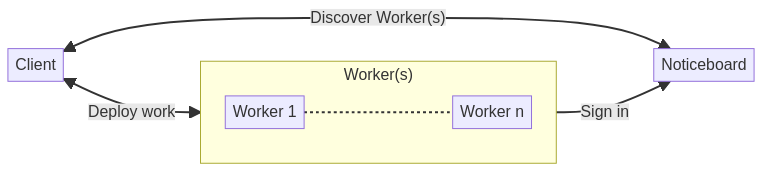
\includegraphics{network-1.png}
        \caption{Caption}
        \label{fig:network-flowchart}
    \end{figure}

    \begin{figure}
        \centering
        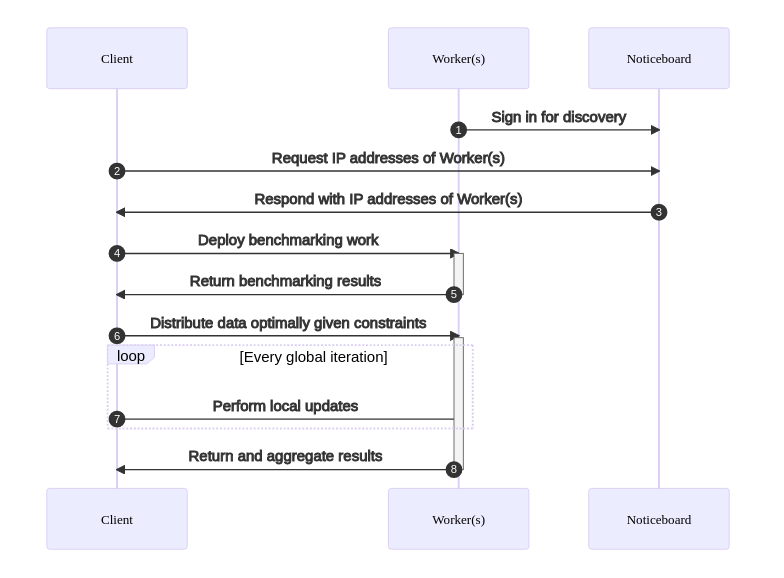
\includegraphics{network-2.png}
        \caption{Caption}
        \label{fig:network-sequence}
    \end{figure}

    \section{Federated Learning}
    \label{sec:Federate-Learning}
\end{document}
